\documentclass[border=1pt]{standalone}
\usepackage[T1]{fontenc}
\usepackage{mathptmx}
\usepackage{pgfplots}
\pgfplotsset{compat=1.18}
\usepgfplotslibrary{groupplots}
\definecolor{cA}{RGB}{31,119,180}\definecolor{cB}{RGB}{230,120,30}\definecolor{cC}{RGB}{44,160,44}
\definecolor{c1}{RGB}{31,119,180}\definecolor{c2}{RGB}{255,127,14}\definecolor{c3}{RGB}{44,160,44}
\definecolor{c4}{RGB}{214,39,40}\definecolor{c5}{RGB}{148,103,189}
\begin{document}

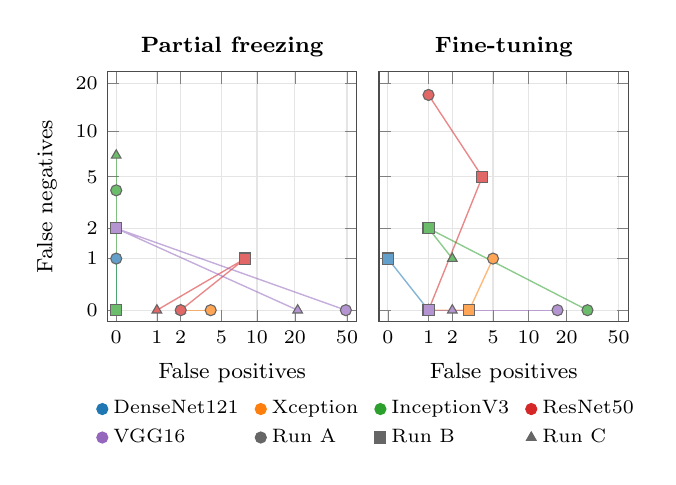
\begin{tikzpicture}
\begin{groupplot}[group style={group size=2 by 1, horizontal sep=8pt, yticklabels at=edge left},
  width=4.75cm, height=4.75cm, xmin=-0.15, xmax=4.1, ymin=-0.15, ymax=3.2,
  xtick={0.0000,0.6931,1.0986,1.7918,2.3979,3.0445,3.9318}, xticklabels={0,1,2,5,10,20,50}, ytick={0.0000,0.6931,1.0986,1.7918,2.3979,3.0445,3.9318}, yticklabels={0,1,2,5,10,20,50},
  ticklabel style={font=\scriptsize}, label style={font=\footnotesize}, title style={font=\footnotesize\bfseries, yshift=-4pt},
  grid=major, grid style={black!10}, axis line style={black!70}, xlabel={False positives},
  legend cell align=left, legend style={font=\scriptsize, draw=none, legend columns=4, at={(1.045,-0.27)}, anchor=north, /tikz/every even column/.append style={column sep=4pt}}]

\nextgroupplot[title={Partial freezing}, ylabel={False negatives}]
\addplot[c1, line width=0.5pt, opacity=0.55, forget plot] coordinates {(0.0000,0.6931) (0.0000,0.0000) (0.0000,0.0000)};
\addplot[only marks, mark=*, mark size=2pt, color=c1, mark options={fill=c1!70, draw=black!60}, forget plot] coordinates {(0.0000,0.6931)};
\addplot[only marks, mark=square*, mark size=2pt, color=c1, mark options={fill=c1!70, draw=black!60}, forget plot] coordinates {(0.0000,0.0000)};
\addplot[only marks, mark=triangle*, mark size=2pt, color=c1, mark options={fill=c1!70, draw=black!60}, forget plot] coordinates {(0.0000,0.0000)};
\addplot[c2, line width=0.5pt, opacity=0.55, forget plot] coordinates {(1.6094,0.0000) (1.0986,0.0000)};
\addplot[only marks, mark=*, mark size=2pt, color=c2, mark options={fill=c2!70, draw=black!60}, forget plot] coordinates {(1.6094,0.0000)};
\addplot[only marks, mark=triangle*, mark size=2pt, color=c2, mark options={fill=c2!70, draw=black!60}, forget plot] coordinates {(1.0986,0.0000)};
\addplot[c3, line width=0.5pt, opacity=0.55, forget plot] coordinates {(0.0000,1.6094) (0.0000,0.0000) (0.0000,2.0794)};
\addplot[only marks, mark=*, mark size=2pt, color=c3, mark options={fill=c3!70, draw=black!60}, forget plot] coordinates {(0.0000,1.6094)};
\addplot[only marks, mark=square*, mark size=2pt, color=c3, mark options={fill=c3!70, draw=black!60}, forget plot] coordinates {(0.0000,0.0000)};
\addplot[only marks, mark=triangle*, mark size=2pt, color=c3, mark options={fill=c3!70, draw=black!60}, forget plot] coordinates {(0.0000,2.0794)};
\addplot[c4, line width=0.5pt, opacity=0.55, forget plot] coordinates {(1.0986,0.0000) (2.1972,0.6931) (0.6931,0.0000)};
\addplot[only marks, mark=*, mark size=2pt, color=c4, mark options={fill=c4!70, draw=black!60}, forget plot] coordinates {(1.0986,0.0000)};
\addplot[only marks, mark=square*, mark size=2pt, color=c4, mark options={fill=c4!70, draw=black!60}, forget plot] coordinates {(2.1972,0.6931)};
\addplot[only marks, mark=triangle*, mark size=2pt, color=c4, mark options={fill=c4!70, draw=black!60}, forget plot] coordinates {(0.6931,0.0000)};
\addplot[c5, line width=0.5pt, opacity=0.55, forget plot] coordinates {(3.9120,0.0000) (0.0000,1.0986) (3.0910,0.0000)};
\addplot[only marks, mark=*, mark size=2pt, color=c5, mark options={fill=c5!70, draw=black!60}, forget plot] coordinates {(3.9120,0.0000)};
\addplot[only marks, mark=square*, mark size=2pt, color=c5, mark options={fill=c5!70, draw=black!60}, forget plot] coordinates {(0.0000,1.0986)};
\addplot[only marks, mark=triangle*, mark size=2pt, color=c5, mark options={fill=c5!70, draw=black!60}, forget plot] coordinates {(3.0910,0.0000)};
\addlegendimage{only marks, mark=*, color=c1}\addlegendentry{DenseNet121}
\addlegendimage{only marks, mark=*, color=c2}\addlegendentry{Xception}
\addlegendimage{only marks, mark=*, color=c3}\addlegendentry{InceptionV3}
\addlegendimage{only marks, mark=*, color=c4}\addlegendentry{ResNet50}
\addlegendimage{only marks, mark=*, color=c5}\addlegendentry{VGG16}
\addlegendimage{only marks, mark=*, color=black!60}\addlegendentry{Run A}
\addlegendimage{only marks, mark=square*, color=black!60}\addlegendentry{Run B}
\addlegendimage{only marks, mark=triangle*, color=black!60}\addlegendentry{Run C}
\nextgroupplot[title={Fine-tuning}]
\addplot[c1, line width=0.5pt, opacity=0.55, forget plot] coordinates {(0.6931,0.0000) (0.0000,0.6931) (0.6931,0.0000)};
\addplot[only marks, mark=*, mark size=2pt, color=c1, mark options={fill=c1!70, draw=black!60}, forget plot] coordinates {(0.6931,0.0000)};
\addplot[only marks, mark=square*, mark size=2pt, color=c1, mark options={fill=c1!70, draw=black!60}, forget plot] coordinates {(0.0000,0.6931)};
\addplot[only marks, mark=triangle*, mark size=2pt, color=c1, mark options={fill=c1!70, draw=black!60}, forget plot] coordinates {(0.6931,0.0000)};
\addplot[c2, line width=0.5pt, opacity=0.55, forget plot] coordinates {(1.7918,0.6931) (1.3863,0.0000) (0.6931,0.0000)};
\addplot[only marks, mark=*, mark size=2pt, color=c2, mark options={fill=c2!70, draw=black!60}, forget plot] coordinates {(1.7918,0.6931)};
\addplot[only marks, mark=square*, mark size=2pt, color=c2, mark options={fill=c2!70, draw=black!60}, forget plot] coordinates {(1.3863,0.0000)};
\addplot[only marks, mark=triangle*, mark size=2pt, color=c2, mark options={fill=c2!70, draw=black!60}, forget plot] coordinates {(0.6931,0.0000)};
\addplot[c3, line width=0.5pt, opacity=0.55, forget plot] coordinates {(3.4012,0.0000) (0.6931,1.0986) (1.0986,0.6931)};
\addplot[only marks, mark=*, mark size=2pt, color=c3, mark options={fill=c3!70, draw=black!60}, forget plot] coordinates {(3.4012,0.0000)};
\addplot[only marks, mark=square*, mark size=2pt, color=c3, mark options={fill=c3!70, draw=black!60}, forget plot] coordinates {(0.6931,1.0986)};
\addplot[only marks, mark=triangle*, mark size=2pt, color=c3, mark options={fill=c3!70, draw=black!60}, forget plot] coordinates {(1.0986,0.6931)};
\addplot[c4, line width=0.5pt, opacity=0.55, forget plot] coordinates {(0.6931,2.8904) (1.6094,1.7918) (0.6931,0.0000)};
\addplot[only marks, mark=*, mark size=2pt, color=c4, mark options={fill=c4!70, draw=black!60}, forget plot] coordinates {(0.6931,2.8904)};
\addplot[only marks, mark=square*, mark size=2pt, color=c4, mark options={fill=c4!70, draw=black!60}, forget plot] coordinates {(1.6094,1.7918)};
\addplot[only marks, mark=triangle*, mark size=2pt, color=c4, mark options={fill=c4!70, draw=black!60}, forget plot] coordinates {(0.6931,0.0000)};
\addplot[c5, line width=0.5pt, opacity=0.55, forget plot] coordinates {(2.8904,0.0000) (0.6931,0.0000) (1.0986,0.0000)};
\addplot[only marks, mark=*, mark size=2pt, color=c5, mark options={fill=c5!70, draw=black!60}, forget plot] coordinates {(2.8904,0.0000)};
\addplot[only marks, mark=square*, mark size=2pt, color=c5, mark options={fill=c5!70, draw=black!60}, forget plot] coordinates {(0.6931,0.0000)};
\addplot[only marks, mark=triangle*, mark size=2pt, color=c5, mark options={fill=c5!70, draw=black!60}, forget plot] coordinates {(1.0986,0.0000)};
\end{groupplot}
\end{tikzpicture}
\end{document}
